\documentclass[9 pt]{article} % For LaTeX2e
\usepackage{nips14submit_e,times}
\usepackage{hyperref}
\usepackage{url}
\usepackage{amsmath,amsfonts}
\usepackage{algorithmic}
\usepackage{algorithm}
\usepackage[caption=false,font=normalsize,labelfont=sf,textfont=sf]{subfig}
\usepackage{textcomp}
\usepackage{stfloats}
\usepackage{xcolor}
\usepackage{verbatim}
\usepackage{graphicx}
\usepackage{cite}
\usepackage{array}
\usepackage{subcaption}
\usepackage{subfigure}
\usepackage[margin=0.75in]{geometry}  
\usepackage{titlesec}
\titleformat{\section}{\large\bfseries}{\thesection}{1em}{}
\titleformat{\subsection}{\normalsize\bfseries}{\thesubsection}{1em}{}
\usepackage{enumitem}
\setlist{noitemsep}  
\setlength{\abovecaptionskip}{2pt}  
\setlength{\belowcaptionskip}{2pt} 
\setlength{\textfloatsep}{5pt}  


% Adjust hyperref package options
\usepackage[colorlinks=true, citecolor=black, linkcolor=blue, urlcolor=blue]{hyperref}

% Disable boxes around links
\hypersetup{
    pdfborder={0 0 0} % Disable boxes around links
}


%\documentstyle[nips14submit_09,times,art10]{article} % For LaTeX 2.09

\title{Modeling Disease Spread and Health Behavior Diffusion through Clustering and Social Network Exposure}


\author{
Divya Aggarwal\thanks{4th year BS-MS Economics, Enrollment Number: 21322011} \\
Humanities and Social Sciences Department\\
Indian Institute of Technology Roorkee \\
Roorkee, Uttarakhand, India \\
\texttt{d\_aggarwal@hs.iitr.ac.in}
}


% The \author macro works with any number of authors. There are two commands
% used to separate the names and addresses of multiple authors: \And and \AND.
%
% Using \And between authors leaves it to \LaTeX{} to determine where to break
% the lines. Using \AND forces a linebreak at that point. So, if \LaTeX{}
% puts 3 of 4 authors names on the first line, and the last on the second
% line, try using \AND instead of \And before the third author name.

\newcommand{\fix}{\marginpar{FIX}}
\newcommand{\new}{\marginpar{NEW}}

\nipsfinalcopy % Uncomment for camera-ready version
\setlength{\parskip}{0pt}
\setlength{\parindent}{1em}  % Optional: Adjust indent as needed

\begin{document}


\maketitle

\begin{abstract}
This report investigates the dynamics of infectious disease transmission, emphasizing the roles of social interactions, demographic factors, and social interactions. By incorporating the concept of Social Network Exposure (SNE) into traditional epidemiological models, the report reveals how weak ties among diverse socioeconomic groups can influence disease spread. It highlights the significance of age-structured approaches in understanding susceptibility and recovery patterns across different cohorts. Additionally, the integration of latent and asymptomatic infection stages captures the effects of social ties on disease dynamics within closely connected communities. The findings underscore the impact of clustered social networks on prolonging infections and sustaining transmission. Collectively, these insights provide a comprehensive understanding of the multifactorial nature of disease spread and inform public health strategies to mitigate health disparities and improve health outcomes across populations.\\
\textbf{Keywords:} Infectious Disease Dynamics; Social Network Exposure; Clustering Coefficient 
\end{abstract}


\section{Introduction}
\label{headings}
The spread of infectious diseases and the persistence of chronic health conditions are complex phenomena shaped by numerous factors, such as socioeconomic status, social connections, and individual health behaviors \cite{berkman2000social}, \cite{marmot2005social}, and \cite{diezroux2001investigating}. Understanding these influences is essential for crafting impactful public health interventions, especially given current global health challenges. This report presents a comprehensive exploration of these dynamics through four distinct analyses, each addressing a critical aspect of disease transmission.

Infectious diseases and chronic health conditions spread through both biological and social pathways. Traditional epidemiological models, like the Susceptible-Infectious-Recovered (SIR) framework \cite{kermack1927contribution}, have long been used to predict disease spread. However, these models often fail to account for the complexity of social networks that influence not only the rate of transmission but also the reach of health behaviors across socioeconomic classes.

The motivation behind this study is to extend these classical models by incorporating Social Network Exposure (SNE) and economic connectedness into the analysis of disease transmission and health behavior diffusion. Specifically, we examine how social structures, particularly cross-class friendships and strong clustering within social groups, impact the dynamics of both infectious diseases and chronic conditions.

Analysis 1: Economic Connectedness and Disease Spread investigates how social and economic ties influence the transmission of infectious diseases. Building on the Strength of Weak Ties Theory by Granovetter \cite{granovetter1973strength}, this analysis introduces the Social Network Exposure (SNE) variable into the Susceptible-Infectious-Recovered (SIR) model \cite{kermack1927contribution}. By analyzing the impact of weak ties among disparate socioeconomic groups, this analysis elucidates how economic connectedness can facilitate or hinder the spread of diseases.

Analysis 2: Age-Structured Models for Understanding Infectious Disease Dynamics \cite{diekmann2013mathematical} emphasizes the importance of demographic factors in shaping infection rates and recovery patterns. This analysis segments populations into distinct age groups, reflecting variations in susceptibility and transmission rates. By utilizing age-structured models, it becomes evident that age-specific interactions significantly influence disease dynamics, thereby informing targeted interventions tailored to vulnerable age cohorts.

Analysis 3: The SLIAR Model \cite{ajelli2010sliar} with Social Network Exposure (SNE) for Infectious Disease Dynamics extends the traditional SIR framework by incorporating both the latent and asymptomatic stages of infection. This model allows for a more nuanced understanding of how social ties and mobility affect disease progression. The inclusion of SNE within the SLIAR model captures the intricate interplay between social interactions and infectious disease dynamics, particularly within closely connected communities.

Analysis 4: Clustered Network Epidemics via Incorporating Social Interactions focuses on the impact of social clustering on disease spread \cite{miller2009percolation}. By examining how infections propagate through clustered networks, this analysis reveals that social interactions significantly alter the trajectories of epidemics. Higher clustering coefficients lead to prolonged infection durations and sustained transmission within tight-knit groups, highlighting the role of community dynamics in shaping public health outcomes.

Together, these analyses provide a comprehensive framework for understanding the complexities of infectious disease transmission. By integrating economic connectedness, demographic factors, and social interactions into traditional epidemiological models, this report aims to inform public health policies that are responsive to the multifactorial nature of disease spread. Through this holistic approach, we can better address health disparities and improve health outcomes across diverse populations.

\section{Summary of the Base Papers}
Raj Chetty et al. have authored two seminal papers examining social capital and its role in economic mobility. The first paper, \textit{Social Capital I: Measurement and Associations with Economic Mobility} \cite{chetty2022social}, focuses on measuring social capital and its link to upward mobility, while the second, \textit{Social Capital II: Determinants of Economic Connectedness} \cite{chetty2022social2}, investigates the factors that shape economic connections across different socioeconomic groups.

\subsection{Social Capital I: Measurement and Associations with Economic Mobility}
\subsubsection*{Defining and Measuring Social Capital}
The authors describe social capital as the 'strength of an individual's connections within their social network and community' and explore three distinct types \cite{chetty2022social}:

\begin{itemize}
    \item \textbf{Economic Connectedness (EC)}: This metric assesses the extent of the connection between individuals from low and high socioeconomic statuses (SES). It is determined by calculating the proportion of high-SES friends among low-SES individuals, adjusted relative to the total proportion of high-SES individuals in the population.
    \item \textbf{Network Cohesiveness}: This examines the structure of social networks, emphasizing the presence of cliques and the degree of mutual friendships. Metrics such as clustering coefficient, support ratio, and spectral homophily are used to quantify these aspects.
    \item \textbf{Civic Engagement}: It can be assessed through factors such as the rate of volunteering, engagement in community organizations, and the degree of trust within the community.
\end{itemize}

\subsubsection*{Key Findings}
\begin{itemize}
    \item \textbf{Geographical Variation}: There is considerable variation in all three social capital measures across different counties in the United States.
    \item \textbf{Economic Connectedness and Mobility}: The study finds a strong positive association between EC and upward income mobility. Children from low-income families who grow up in areas with higher EC tend to have higher incomes in adulthood. The study suggests that if children from low-SES families were raised in counties with EC compared to those experienced by the average child from high-SES parents, their future incomes would increase by an average of 20\%. This factor stands out as one of the most significant predictors of upward economic mobility.
    \item \textbf{Other Social Capital Measures}: Network cohesiveness and civic engagement measures show weaker and less consistent correlations with economic mobility. For example, while civic engagement tends to be higher in rural areas, its correlation with economic mobility becomes weaker once the data is weighted to account for the greater concentration of low-income families in urban communities.
\end{itemize}

\subsection{Social Capital II: Determinants of Economic Connectedness}
This paper expands on the first paper by concentrating specifically on the factors that influence Economic Connectedness (EC), which is the form of social capital most closely associated with economic mobility. \cite{chetty2022social2}

\subsubsection*{Decomposing Economic Connectedness}
The authors distinguish between two key mechanisms that drive differences in EC:

\begin{itemize}
    \item \textbf{Exposure}: The extent to which individuals from different SES backgrounds are present in the same social settings (e.g., schools, religious organizations, workplaces). The study reveals that around half of the disparity in Economic Connectedness (EC) between individuals from low and high-SES backgrounds can be attributed to differences in their exposure.
    \item \textbf{Friending Bias}: The tendency for individuals to form friendships with others from similar SES backgrounds, even when controlling for the level of exposure to people from different SES groups within a given setting. The study finds that the bias in forming friendships is more evident in larger, more diverse high schools.
\end{itemize}

\subsubsection*{Key Findings}
\begin{itemize}
    \item \textbf{Exposure and Bias Contribute Equally}: Both exposure and friending bias are key factors in influencing Economic Connectedness (EC), with each accounting for approximately half of the variation in the proportion of high-SES friends between low and high SES individuals.
    \item \textbf{Context Matters}: The extent of friending bias differs significantly across various social environments. For example, friending bias is generally less pronounced in religious organizations than in schools or workplaces.
\end{itemize}

\subsubsection*{Policy Implications}
\begin{itemize}
    \item \textbf{Integration for Low Bias}: In settings with low friending bias, increasing socioeconomic integration (exposure) can effectively boost EC.
    \item \textbf{Addressing Bias Directly}: In settings with high friending bias, interventions should focus on reducing bias within existing groups to promote cross-SES friendships.
\end{itemize}

\section{Related Work}

\cite{doi:10.1073/pnas.1821298116} analyzed the effect of reactive school closures on influenza spread by collecting contact diaries from 259 students and their households in Tomsk, Russia, modeling reduced transmission during school closures. Participants recorded daily contacts in three categories: (i) demographic information, (ii) contact patterns on regular school/workdays, and (iii) contact patterns during school closures. \cite{doi:10.1073/pnas.1811115115} assessed the limitations of the basic reproduction number \( R_0 \) in heterogeneous populations using multiplex networks and SIR models, proposing the time-varying \( R(t) \) for a more accurate representation of epidemic dynamics. \cite{doi:10.1073/pnas.1620161114} applied a global stochastic epidemic model to investigate the transmission of Zika throughout the Americas, showing that mosquito dynamics, mobility, and seasonal factors influenced the outbreak's spatial and temporal patterns. The study utilizes the Global Epidemic and Mobility Model (GLEAM), a stochastic, agent-based framework that uses high-resolution data for various population layers, including households, schools, workplaces, and communities. \cite{trentini2021modeling} studied SARS-CoV-2 transmission in Ethiopia, finding higher infection rates in urban areas but more severe cases in rural regions, linking socio-demographic factors to disease burden in sub-Saharan Africa. \cite{xuan2021discrete} explored how opinion dynamics on disease severity impact infection spread in networks using a discrete-time SIS model, highlighting the role of social factors in epidemiological models.

\cite{miller2009percolation} examined epidemic spread in clustered networks, finding that clustering increases the epidemic threshold by reducing component sizes and transmission pathways compared to unclustered networks. \cite{trevisin2023spatially} proposed a method for estimating spatially explicit reproduction numbers \( R_k(t) \) by incorporating mobility dynamics, improving epidemic modeling with real COVID-19 data from Italy.
\cite{davis2021cryptic} revealed that SARS-CoV-2 spread undetected in early 2020 due to limited testing, with international travel driving early introductions. By March, only 1–3\% of infections were detected in the US and Europe. \cite{cantarelli2014representativeness} found demographic biases in the Influenzanet surveillance network, with underrepresentation of certain age groups, smokers, and diabetics impacting the generalizability of influenza surveillance data. \cite{salje2016how} studied chikungunya transmission in Bangladesh, highlighting the significant role of household-level social interactions, with gender differences and proximity being key factors in infection risk. The study integrates detailed epidemiological data with statistical modeling to assess various risk factors associated with disease transmission.

\section{Data and Measures}
\subsection{Data}
The dataset in the base papers \cite{chetty2022social} and \cite{chetty2022social2} focuses on friendship links among Facebook users between the ages of 25 and 44 living in the United States. The dataset encompasses 21 billion friendship pairs, representing a significant portion of the U.S. population within that age range. The authors use this data to assess different aspects of social capital, such as economic connectedness, network cohesion, and civic participation. The study focuses on this age group because their Facebook usage rate exceeds 80\%, surpassing other age groups, and aligns with readily available demographic data from the American Community Survey (ACS), allowing for comparisons with the broader population.

\textbf{User Information:} In addition to friendship links, the researchers extract data from users' Facebook profiles, which includes self-reported information on several variables such as age, location (ZIP code and county), language, relationship status, educational attainment, gender, college attended, donations made, phone model price, usage of Facebook on different devices (mobile vs. internet), familial ties, mobile carrier, and group memberships. The researchers integrate these variables to create a socioeconomic status (SES) measure for each user.

\textbf{Parental SES and Group-Level Data:} To estimate family SES during childhood, the authors connect individuals in their primary dataset to their parents by utilizing self-reported family relationships, a hashed version of users' last names, and publicly accessible posts and significant life events. In order to examine the social context of connections, the researchers classify friendships into various social settings based on common affiliations, such as high schools, universities, workplaces, neighborhoods (ZIP codes), religious groups, and recreational organizations.

\textbf{External Datasets:} In addition to the Facebook data, the studies incorporate a range of publicly accessible datasets, such as the American Community Survey (ACS), which is used to benchmark the sample and gather information on median incomes by block group, racial and ethnic composition, and other community features. The Opportunity Atlas offers data on intergenerational income mobility, high school graduation rates, and teenage birth rates. School-level data is sourced from the National Center for Education Statistics (NCES) and the Civil Rights Data Collection (CRDC), while the Integrated Postsecondary Education Data System (IPEDS) provides college-level data. Additionally, Census Data is used to identify the number of individuals with below-national-median parental income, which informs the weighting of correlations and regressions. 

\subsection{Statistical Analysis} This report primarily focuses on theoretical frameworks to understand the dynamics of infectious disease transmission. Simulations have been conducted to illustrate the model outcomes and validate the theoretical constructs. The simulations were implemented using Python, with the accompanying code provided in the attached folder. This computational approach allows for the exploration of various scenarios and the assessment of the impact of different variables on disease dynamics. The authors calculated the exposure and clustering coefficient, which are utilized in this paper.

\subsection{Measures}

\begin{itemize}
    \item \textbf{Infection Population:} Represented by the number of individuals actively infected at a specific point in time.
    
    \item \textbf{Susceptible Population:} Refers to the individuals who are not currently infected but are vulnerable to contracting the disease.
    
    \item \textbf{Latent Period:} The period in which individuals are infected but have not yet become contagious. This period is crucial for understanding the dynamics of disease spread.
    
    \item \textbf{Social Network Exposure (SNE):} Quantified based on the density of social ties within communities, measured through network analysis techniques. The SNE varies between 0 and 1, with higher values signifying stronger social and economic connectedness.
    
    \item \textbf{Clustering Coefficient:} Calculated to assess the degree of interconnectedness among individuals within social networks. Similar to the SNE, the clustering coefficient spans from 0 to 1, where higher values indicate more closely-knit social groups.
\end{itemize}

\section{Theoretical Frameworks}
\subsection{Analysis 1: Economic Connectedness and Disease Spread}

\textbf{Existing Theory: The Strength of Weak Ties} \\
Strength of Weak Ties theory (1973) by Granovetter \cite{granovetter1973strength} is foundational in social network research, positing that weak ties between disparate groups are critical for the diffusion of information. These weak ties, typically characterized as connections between individuals from different socioeconomic backgrounds, provide a bridge for sharing new ideas, knowledge, and opportunities that would otherwise remain isolated within homogeneous groups.

In the context of disease transmission, this theory can be adapted to highlight how cross-class friendships (weak ties) facilitate faster and broader disease spread by connecting different socioeconomic groups. When applied to an epidemiological framework, weak ties serve as conduits through which infections can travel across the otherwise disconnected clusters of social groups, thereby increasing the overall exposure in a population. Conversely, strong homophily (friending bias), where people preferentially form relationships within their own social and economic class, limits this cross-group transmission and results in more contained outbreaks.

\textbf{Extension: Social Network Exposure (SNE) in the SIR Model} \\
To examine how economic connectedness influences disease transmission, we introduce a Social Network Exposure (SNE) variable into the classical SIR (Susceptible-Infectious-Recovered) model. This variable measures the level of interaction between individuals from different socioeconomic backgrounds, capturing the economic connectedness across social classes. By modifying the infection rate based on this level of social interaction, we are able to model how cross-class friendships influence the overall dynamics of infectious disease spread.

The SIR model \cite{kermack1927contribution} describes the evolution of three key population groups:
\begin{itemize}
    \item Susceptible (S): Individuals who are at risk of contracting the disease.
    \item Infected (I): Individuals who are currently infected and capable of spreading the disease.
    \item Recovered (R): Individuals who have recovered from the disease and are immune to reinfection.
\end{itemize}

The higher the \textbf{SNE} value, the more frequent the interactions between different socioeconomic groups, leading to increased disease spread. Conversely, lower \textbf{SNE} indicates higher friending bias, where cross-class interactions are limited, resulting in fewer cross-group infections. The equations are adjusted as follows:

1. \textbf{Modified Susceptible Population}:
   \[
   \frac{ds(t)}{dt} = -\beta \cdot k \cdot \text{SNE} \cdot i(t) \cdot [1 - r(t) - i(t)]
   \]
   Where:
    \begin{itemize}
        \item \(s(t)\): The fraction of the population that is susceptible at time \(t\).
        \item \(\beta\): The infection rate, representing the likelihood of disease transmission per contact. 
        \item \(k\): The average number of interactions an individual has.
        \item \(i(t)\): The fraction of the population that is infected at time \(t\).
        \item \(r(t)\): The fraction of the population that has recovered from the disease.
    \end{itemize}
   The SNE modifies the infection rate based on the degree of cross-class interactions, increasing transmission as economic connectedness rises.

2. \textbf{Modified Infected Population}:
   \[
   \frac{di(t)}{dt} = \beta \cdot k \cdot \text{SNE} \cdot i(t) \cdot [1 - r(t) - i(t)] - \mu \cdot i(t)
   \]
   Where:
   \begin{itemize}
       \item \(\mu\): Recovery rate, indicating how quickly infected individuals recover.
   \end{itemize}
   The infection term now reflects the influence of SNE, where higher cross-class interactions boost the probability of infected individuals contracting the disease \cite{nunner2021model}.

3. \textbf{Recovered Population}:
   \[
   \frac{dr(t)}{dt} = \mu \cdot i(t)
   \]
   Where:
   \begin{itemize}
       \item \(r(t)\): Fraction of the population that has recovered at time \(t\).
   \end{itemize}

\subsection{Analysis 2: Age-Structured Models for Understanding Infectious Disease Dynamics}

Age-structured models \cite{diekmann2013mathematical} are essential in infectious disease research as they consider the variation in transmission rates, susceptibility, and recovery across different age groups. These models are vital for understanding how diseases spread in populations with heterogeneous contact patterns and immune responses. By segmenting populations by age, these models provide a detailed insight into disease behavior and facilitate the creation of more focused intervention strategies.

\textbf{Key Components of Age-Structured Models:}

1. \textbf{Population Segmentation:} \\
   The population is divided into distinct age groups, or cohorts, each with unique characteristics related to:
   \begin{itemize}
       \item \textbf{Infection Rates:} Younger individuals may have higher rates of contact, such as through schools, and thus higher transmission potential, while older individuals may be more vulnerable to severe outcomes.
       \item \textbf{Recovery Rates:} Recovery can vary with age due to immune system differences, with younger individuals often recovering faster than older ones.
       \item \textbf{Contact Patterns:} The model accounts for how different age groups interact with one another, with children, for example, having more frequent close contact with peers, while older individuals may have fewer but more high-risk interactions.
   \end{itemize}

2. \textbf{Dynamic Interactions:} \\
   Age-structured models simulate the interactions between these age groups, allowing researchers to study how a disease spreads through the different cohorts over time based on varying infection and recovery rates.

\textbf{Basic Structure of Age-Structured Models} \\
The population is divided into several age classes, denoted as \( A_1, A_2, \ldots, A_n \), where each class \( A_i \) represents a specific age range (e.g., 0-5 years, 6-15 years, 16-59 years, 60+ years). The model typically uses a compartmental approach for each age group, with individuals classified into infectious (I), susceptible (S), and recovered (R) compartments.

\textbf{Equations of Age-Structured Models}

1. \textbf{Susceptible Population:}
   \[
   \frac{dS_i}{dt} = -\beta_i S_i \sum_{j} \left( \frac{I_j}{N_j} \right) \cdot C_{ij}
   \]
The variable \( S_i \) represents the count of individuals in age group \( A_i \) who are susceptible to the disease. \( \beta_i \) denotes the transmission rate specific to age group \( A_i \). \( I_j \) refers to the count of individuals in age group \( A_j \) who are currently infected. The element \( C_{ij} \) of the contact matrix quantifies the interaction rates between age groups \( A_i \) and \( A_j \).

   \[
   C_{ij} = SNE_{ij}
   \]
   Where:
   - \( SNE_{ij} \): The Social Network Exposure factor that quantifies the level of cross-class interaction between age groups \( A_i \) and \( A_j \). Higher values indicate more interaction and greater economic connectedness.

2. \textbf{Infectious Population:}
   \[
   \frac{dI_i}{dt} = \beta_i S_i \sum_{j} \left( \frac{I_j}{N_j} \right) \cdot C_{ij} - \gamma_i I_i
   \]
The variable \( I_i \) represents the number of individuals in age group \( A_i \) who are infectious. \( \gamma_i \) denotes the recovery rate for age group \( A_i \).

3. \textbf{Recovered Population:}
   \[
   \frac{dR_i}{dt} = \gamma_i I_i
   \]
   - \( R_i \): The count of individuals in age group \( A_i \) who have recovered.

These equations describe the transitions between susceptible, infected, and recovered states within each age group, while the contact matrix \( C \) captures the interactions between different age groups, influencing the spread of the disease.

\textbf{Matrix Representation of the Model} \\
In matrix form, the system of equations can be represented as:

\[
\mathbf{X} = \begin{bmatrix} S_1 \\ S_2 \\ \vdots \\ S_n \\ I_1 \\ I_2 \\ \vdots \\ I_n \\ R_1 \\ R_2 \\ \vdots \\ R_n \end{bmatrix}
\quad \text{and} \quad \mathbf{C} = \begin{bmatrix} C_{11} & C_{12} & \ldots & C_{1n} \\ C_{21} & C_{22} & \ldots & C_{2n} \\ \vdots & \vdots & \ddots & \vdots \\ C_{n1} & C_{n2} & \ldots & C_{nn} \end{bmatrix}
\]

The contact matrix \( \mathbf{C} \) represents the rates of interaction between various age groups, influencing the transmission of the disease.

The system of equations can be summarized as follows:

\[
\frac{d\mathbf{X}}{dt} = \mathbf{A}(\mathbf{X}) - \mathbf{B}(\mathbf{X})
\]

Where \( \mathbf{A} \) represents the infection dynamics, and \( \mathbf{B} \) represents the recovery dynamics.


\subsection{Analysis 3: SLIAR Model with Social Network Exposure (SNE) for Infectious Disease Dynamics}

The SLIAR model \cite{ajelli2010sliar} is an extension of the traditional SIR (Susceptible-Infectious-Recovered) framework that incorporates additional compartments to account for the latent and asymptomatic stages of infection. This model allows for a more nuanced understanding of how infectious diseases spread, particularly in populations where asymptomatic individuals play a significant role.

\textbf{1. Compartment Definitions}

The SLIAR model includes the following compartments:

\begin{itemize}
    \item \textbf{S (Susceptible):} Individuals who are not infected and can become infected.
    \item \textbf{L (Latent):} Individuals who have contracted the disease but are not yet able to transmit it. They cannot transmit the disease to others during this latent period but will eventually progress to the infectious state.
    \item \textbf{I (Infectious Symptomatic):} Individuals who are infected and exhibit symptoms. These individuals can spread the disease to susceptible individuals.
    \item \textbf{A (Infectious Asymptomatic):} Individuals who are infected but do not show symptoms. They can still transmit the disease, often without being aware of their infection.
    \item \textbf{R (Removed):} Individuals who have either recovered from the disease and developed immunity or who have passed away. They can no longer spread the disease.
\end{itemize}

\textbf{2. Modification of the SLIAR Model with Social Network Exposure (SNE)}

To incorporate Social Network Exposure (SNE) into the SLIAR model, we modify the equations to account for how social interactions influence disease transmission dynamics. The SNE variable reflects the degree of cross-class interactions within the community, affecting the infection rates.

\textbf{Modified SLIAR Model Equations:}

1. \textbf{Susceptible Population:}
   \[
   \frac{dS}{dt} = -\beta S \left(I + \delta A\right) \cdot SNE, \quad S(0) = S_0 > 0
   \]
SNE represents a factor that quantifies social network exposure, with higher values indicating more interaction and thus a greater chance of infection \cite{nunner2021model}. The parameter \(\beta\) refers to the transmission rate, while \(I\) denotes infectious symptomatic individuals. The term \(A\) represents infectious asymptomatic individuals, and \(\delta\) is a factor that accounts for the increased risk of infection posed by asymptomatic individuals.

2. \textbf{Latent Population:}
   \[
   \frac{dL}{dt} = \beta S \left(I + \delta A\right) \cdot SNE - \kappa L, \quad L(0) = L_0 \geq 0
   \]
The latent individuals' infection dynamics are also influenced by the SNE factor. The parameter \(\kappa\) represents the rate at which individuals transition from the latent phase to the infectious phase.

3. \textbf{Infectious Symptomatic Population:}
   \[
   \frac{dI}{dt} = p \kappa L - \alpha I, \quad I(0) = I_0 \geq 0
   \]
The parameter \(p\) represents the proportion of latent individuals who become symptomatic, while \(\alpha\) is the recovery rate for symptomatic individuals. This equation remains unchanged as the progression of symptomatic individuals is not directly influenced by the SNE.

4. \textbf{Infectious Asymptomatic Population:}
   \[
   \frac{dA}{dt} = (1 - p) \kappa L - \eta A, \quad A(0) = A_0 \geq 0
   \]
The parameter \(\eta\) represents the recovery rate for asymptomatic individuals. This equation also remains unchanged.

5. \textbf{Removed Population:}
   \[
   \frac{dR}{dt} = f \alpha I + \eta A, \quad R(0) = R_0 \geq 0
   \]
The parameter \(f\) denotes the proportion of symptomatic individuals who transition to the removed class due to recovery or death. This equation also remains unchanged.

6. \textbf{Total Population:}
   \[
   N(t) = S(t) + L(t) + I(t) + A(t) + R(t)
   \]

The inclusion of SNE modifies the transmission dynamics for both the Susceptible and Latent compartments. By capturing the effect of varying degrees of social interactions and economic connectedness, the model better reflects real-world disease dynamics.


\subsection{Analysis 4: Clustered Network Epidemics via Incorporating Social Interactions}

This approach is particularly relevant in studying how social interactions influence the spread of infectious diseases among closely-knit groups \cite{miller2009percolation}. Here, the clustering coefficient is used.

\textbf{1. Infection Probability in a Triangle (Social Group)}

The model treats nodes \( u, v, \) and \( w \) as members of a triangular social group, representing tight-knit relationships such as family, friends, or coworkers. This configuration captures how infections spread among interconnected individuals.

\textbf{Infection Probabilities:}
- \textbf{Both Neighbors Infected}:
  \[
  P(\text{infect both}) = C \cdot (3T^2 - 2T^3)
  \]
- \textbf{Exactly One Neighbor Infected}:
  \[
  P(\text{infect one}) = 2T(1 - T)^2
  \]
- \textbf{Neither Neighbor Infected}:
  \[
  P(\text{infect none}) = (1 - T)^2
  \]

Here, \( T \) is the transmissibility, reflecting the probability of infection occurring along an edge. The clustering coefficient \( C \) enhances the likelihood of simultaneous infections within these close-knit groups.

\textbf{Expected Number of Infections:} The expected number of infections per triangle can be computed as follows:
\[
E[\text{Infections}] = 2T(1 - T)^2 + 2C(3T^2 - 2T^3) = 2T + 4T^2 - 4T^3 + 6CT^2 - 4CT^3
\]

This equation illustrates the dependence of infection spread on both transmissibility \( T \) and the clustering coefficient \( C \).

\textbf{2. Next-Generation Matrix for Social Network Exposure (SNE)}

To capture the transmission dynamics through different pathways—independent edges and triangle edges—a next-generation matrix is defined:

\[
\begin{bmatrix}
n_I(s+1) \\
n_\Delta(s+1)
\end{bmatrix}
=
\begin{bmatrix}
c_{II} & c_{I\Delta} \\
c_{\Delta I} & c_{\Delta \Delta}
\end{bmatrix}
\begin{bmatrix}
n_I(s) \\
n_\Delta(s)
\end{bmatrix}
\]

Where:
- \( n_I(s) \): Number of nodes infected through independent edges.
- \( n_\Delta(s) \): Number of nodes infected through triangle edges.

\textbf{Calculating the Matrix Elements:}
1. Infection along Independent Edges:
   \[
   c_{II} = T \cdot \frac{\langle K_I^2 - K_I \rangle}{\langle K_I \rangle}
   \]
   
2. Infection along Triangle Edges from Independent Edges:
   \[
   c_{I\Delta} = (2T + 4T^2 - 4T^3 + 6CT^2 - 4CT^3) \cdot \frac{\langle K_I K_\Delta \rangle}{\langle K_I \rangle}
   \]
   
3. Infection along Independent Edges from Triangle Edges:
   \[
   c_{\Delta I} = T \cdot \frac{\langle K_I K_\Delta \rangle}{\langle K_\Delta \rangle}
   \]
   
4. Infection along Triangle Edges:
   \[
   c_{\Delta \Delta} = (2T + 4T^2 - 4T^3 + 6CT^2 - 4CT^3) \cdot \frac{\langle K_\Delta^2 - K_\Delta \rangle}{\langle K_\Delta \rangle}
   \]

These matrix elements capture the pathways through which infections spread and highlight the importance of both individual and clustered interactions in the overall transmission dynamics.

\textbf{3. Basic Reproduction Number and Critical Transmissibility}

The basic reproduction number, \( R_0 \), is a crucial epidemiological metric that indicates the potential for disease spread. It is determined from the dominant eigenvalue of the next-generation matrix, which models the transmission dynamics of the infection. If \( R_0 \) exceeds 1, it suggests that the infection has the potential to spread through the population. Conversely, when \( R_0 \) is less than 1, it implies that the disease will eventually fade out.

\section{Results}

\subsection{Analysis 1: Economic Connectedness and Disease Spread}

The simulation of the SIR model with Social Network Exposure (SNE), as shown in Figure \ref{analysis_1_sne_1}, was conducted using Python with a total population of 1,000 individuals. Initially, there was one infected individual and 0 recovered individuals, resulting in 999 susceptible individuals. The contact rate (\(\beta\)) was set at 0.2, while the mean recovery rate (\(\gamma\)) was \(1/10\), indicating an average recovery time of 10 days. The SNE factor was fixed at 1, reflecting maximum social network exposure. The simulation spanned 160 days, with time points generated at 1-day intervals using `numpy.linspace`. The SIR model equations were modified to incorporate SNE and the resulting differential equations were solved using the `odeint` function from the `scipy.integrate` library to assess the impact of social interactions on disease dynamics. Figure \ref{analysis_1_sne_change} is obtained by changing SNE. 

\begin{figure}[h]
    \centering
    \begin{minipage}[t]{0.45\textwidth}
        \centering
        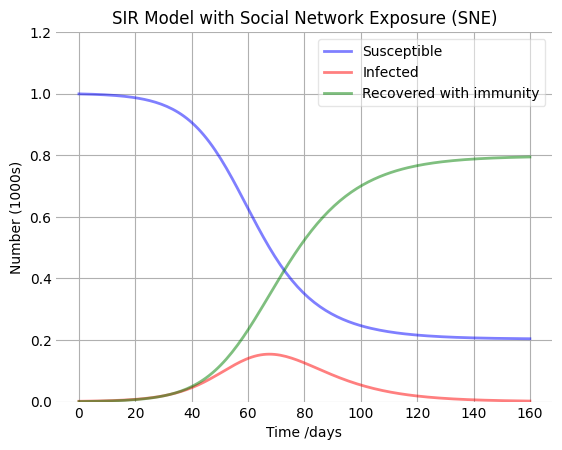
\includegraphics[height=5cm]{Figures/SNE_1_analysis_1.png}
        \caption{SIR Model with Social Network Exposure (SNE) =1}
        \label{analysis_1_sne_1}
    \end{minipage}
    \hspace{0.05\textwidth}
    \begin{minipage}[t]{0.45\textwidth}
        \centering
        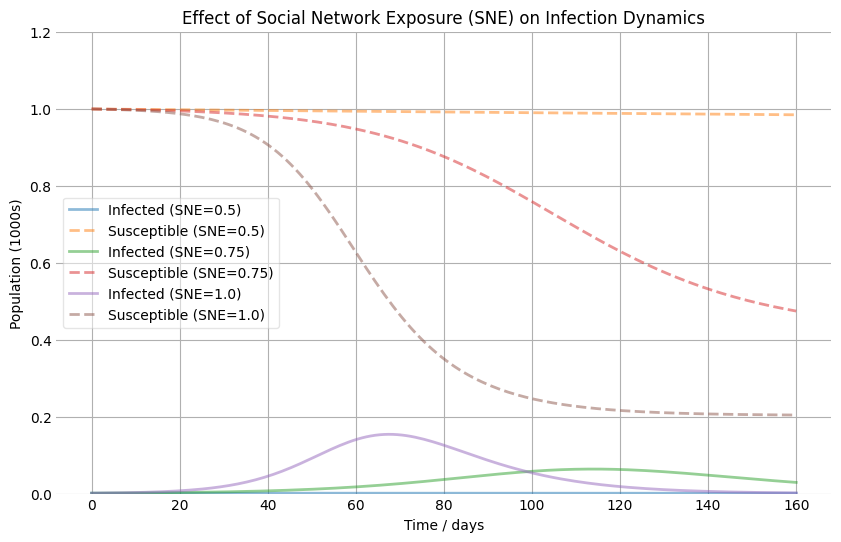
\includegraphics[height=5cm]{Figures/changing_SNE_Analysis_1.png}
        \caption{Effect of Social Network Exposure (SNE) on Infection Dynamics}
        \label{analysis_1_sne_change}
    \end{minipage}
\end{figure}

In regions with high economic connectedness (low friending bias), the disease spreads rapidly across socioeconomic groups, leading to an earlier peak in infections and a faster decline in susceptible individuals, as shown in Figure \ref{analysis_1_sne_change}. This accelerated transmission strains healthcare resources sooner, requiring prompt interventions. Conversely, in areas with high friending bias (low economic connectedness), outbreaks are more localized within socioeconomic groups, resulting in slower, stratified transmission. This delays the infection peak and causes a more gradual decline in susceptible individuals.

\subsection{Analysis 2: Age-Structured Models for Understanding Infectious Disease Dynamics}

The age-structured model simulation, as shown in Figure \ref{analysis_2_sne_1}, was executed using Python with a total population of 1,000 individuals, evenly divided between two age groups: young and old. Initial conditions included one infected individual in each age group, with zero recovered individuals. The susceptible populations were calculated as follows: the young susceptible population was set to \(S_y = 499\) (i.e., half of the population minus the infected), and the old susceptible population was set to \(S_o = 499\). Contact rates varied between age groups, with the transmission rate for the young set at 0.3 and for the old at 0.1. The mean recovery rate for both groups was defined as \(\frac{1}{10}\) and \( \frac{1}{10}\) respectively, indicating an average recovery period of 10 days.
The Social Network Exposure (SNE) factor was fixed at 1, signifying maximum exposure. The simulation ran for 160 days, using time points generated at 1-day intervals with `numpy.linspace`. The resulting differential equations were solved using the `odeint` function from the `scipy.integrate` library, allowing for the assessment of disease dynamics across age groups and the influence of social interactions. Figure \ref{analysis_2_sne_change} is obtained by changing SNE. 

\begin{figure}[h]
    \centering
    \begin{minipage}[t]{0.45\textwidth}
        \centering
        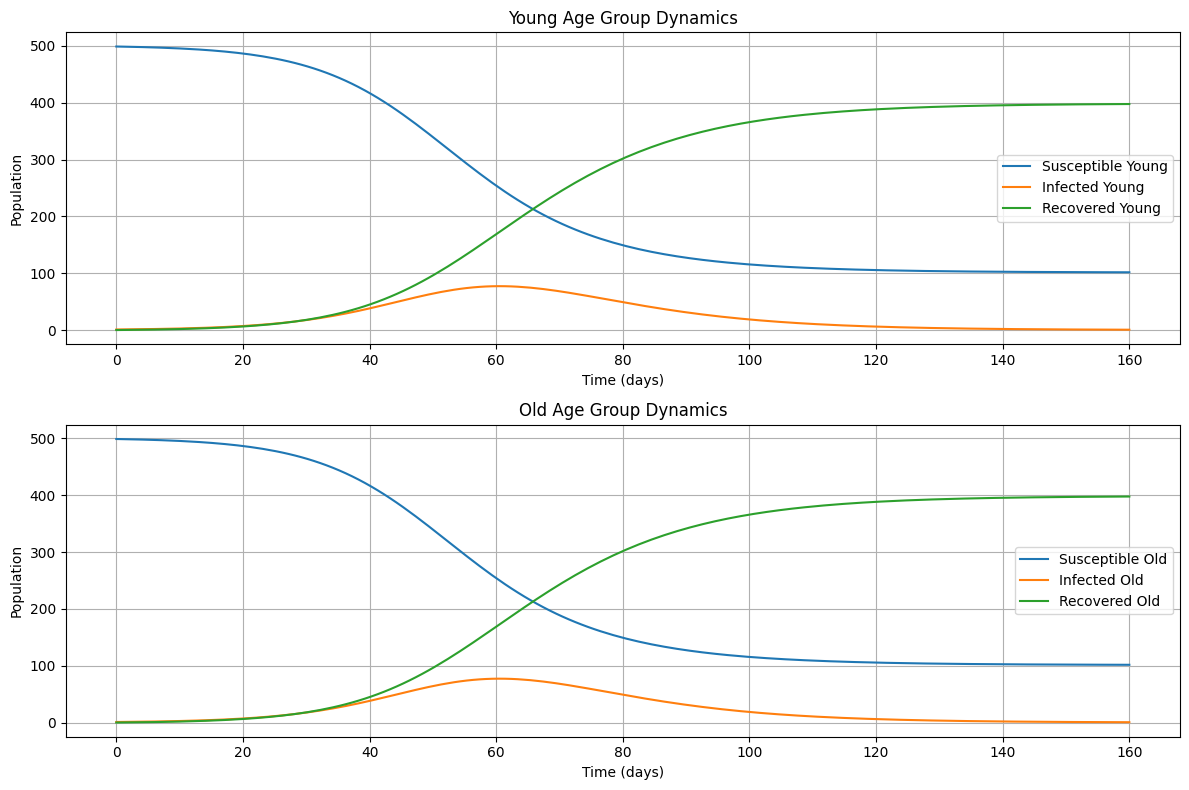
\includegraphics[height=5cm]{Figures/age-wise_SNE_1.png}
        \caption{SIR Model with Young and Old Age Group Dynamics with Social Network Exposure (SNE) =1}
        \label{analysis_2_sne_1}
    \end{minipage}
    \hspace{0.05\textwidth}
    \begin{minipage}[t]{0.45\textwidth}
        \centering
        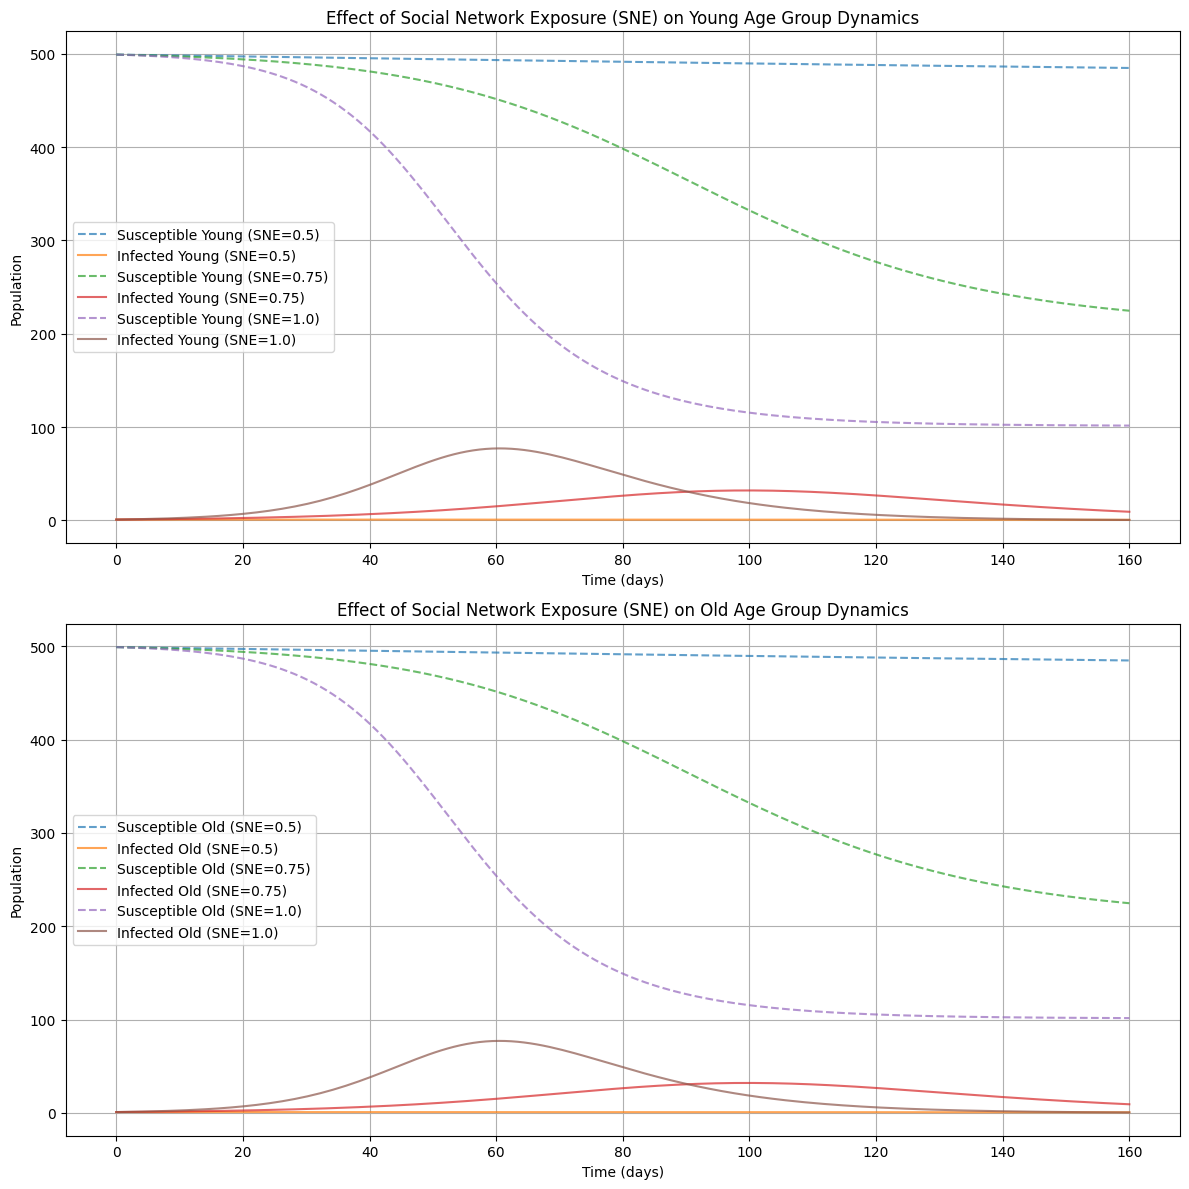
\includegraphics[height=5cm]{Figures/agewise_change_SNE.png}
        \caption{Effect of Social Network Exposure (SNE) on Infection Dynamics in Young and Old Age Group SIR Model}
        \label{analysis_2_sne_change}
    \end{minipage}
\end{figure}

Higher Social Network Exposure (SNE) increases cross-class interactions, leading to faster disease transmission and earlier infection peaks across age groups, as shown in Figure \ref{analysis_2_sne_change}. This acceleration of transmission is particularly evident when younger individuals, often in schools or community settings, have more frequent contact with older adults, heightening the risk of rapid disease spread. As a result, public health systems must prepare for surges in cases earlier than anticipated, requiring swift response measures. Additionally, changes in SNE can highlight vulnerabilities in certain age groups, especially older adults who may be exposed to younger, asymptomatic carriers. The distribution of risk shifts accordingly, necessitating targeted monitoring and intervention. Conversely, lower SNE limits interactions across socioeconomic groups, leading to more localized outbreaks. While this can make containment strategies more straightforward, it may also strain local healthcare resources if not managed effectively.

\subsection{Analysis 3: SLIAR Model with Social Network Exposure (SNE) for Infectious Disease Dynamics}

The simulation of the SLIAR model with Social Network Exposure (SNE), as shown in Figure \ref{analysis_3_sne_1}, was conducted using Python, employing a transmission rate of 0.5 and an infectivity reduction rate for asymptomatic individuals set at 0.3. The transition rate from latent to infected was defined as 0.1, while the recovery rate for symptomatic infections was set at 0.2. The proportion of latent individuals progressing to symptomatic infections was established at 0.6, with a recovery rate for symptomatic individuals fixed at 0.95. Asymptomatic individuals had a recovery rate of 0.1. The SNE factor was fixed at 1.0, indicating full exposure. Initial conditions included 99\% of the population as susceptible, 1\% as latent, and none as symptomatic, asymptomatic, or recovered. The simulation spanned 160 days, with time points generated at 1-day intervals, and the differential equations were solved using the `odeint` function from the `scipy.integrate` library. Figure \ref{analysis_3_sne_change} is obtained by changing SNE. 

\begin{figure}[h]
    \centering
    \begin{minipage}[t]{0.45\textwidth}
        \centering
        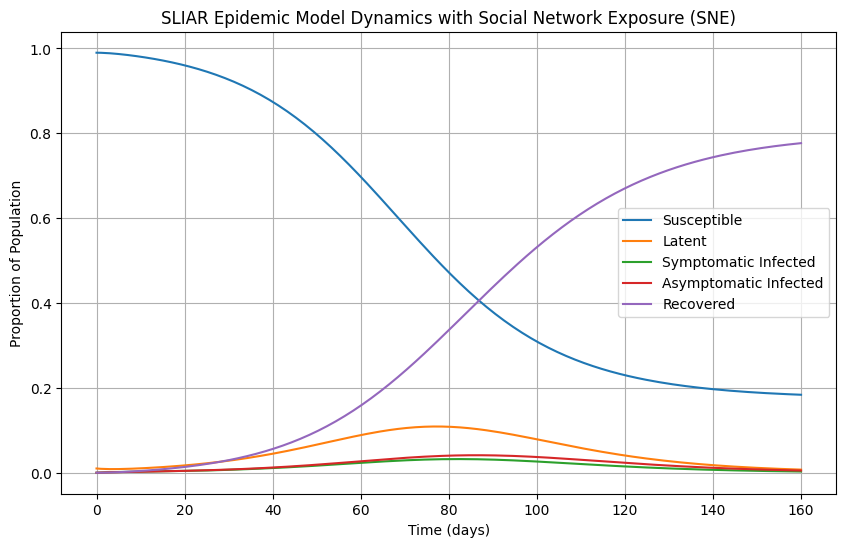
\includegraphics[width=\linewidth]{Figures/anyalsis-3_sne_1.png}
        \caption{SLIAR Epidemic Model Dynamics with Social Network Exposure (SNE) = 1}
        \label{analysis_3_sne_1}
    \end{minipage}
    \hspace{0.05\textwidth}
    \begin{minipage}[t]{0.45\textwidth}
        \centering
        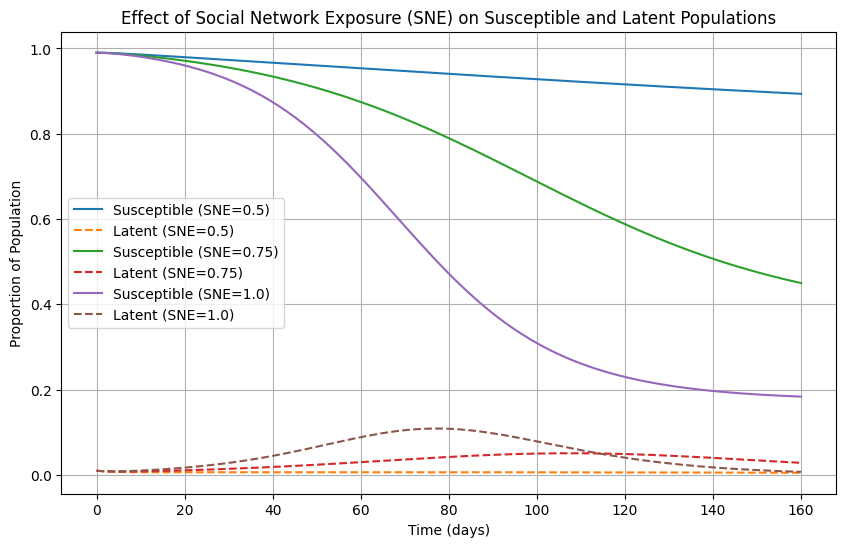
\includegraphics[width=\linewidth]{Figures/analysis_3_sne_chnage.png}
        \caption{Effect of Social Network Exposure (SNE) on SLIAR Epidemic Model Dynamics}
        \label{analysis_3_sne_change}
    \end{minipage}
\end{figure}

Higher Social Network Exposure (SNE) leads to more frequent interactions across socioeconomic groups, resulting in increased infection rates as individuals rapidly move from the susceptible (S) to latent (L) and infectious (I, A) compartments, as shown in Figure \ref{analysis_3_sne_change}. This accelerates disease transmission, particularly among asymptomatic carriers, and drives an earlier peak in infections, putting additional pressure on healthcare systems. Shortened latent and infectious periods further speed up the spread, while asymptomatic individuals contribute significantly to undetected transmission. Different age groups face varying vulnerabilities, with younger populations becoming key transmitters. High SNE also leads to localized outbreaks across socioeconomic groups, complicating containment efforts, whereas low SNE confines outbreaks within specific classes. This stratification may result in disparities in infection and recovery outcomes.

\subsection{Analysis 4: Clustered Network Epidemics via incorporating social interactions}

For Figure \ref{analysis_4_sne_1}, a clustered network consisting of 1,000 nodes was generated, where the probability of forming triangle connections was set at 0.3. The degree distribution for independent edges was modeled using a Poisson distribution with a mean of 2, while triangle edges had a mean of 1. The probability of infection was set at 0.1, while the recovery probability was 0.05. One node was randomly selected as the initial infected individual, and the simulation was run for a maximum of 100-time steps, plotting the number of infected, susceptible, and recovered individuals over time. For Figure \ref{analysis_4_sne_change}, the same parameters were used, but the clustering coefficient of the network was explicitly incorporated into the infection dynamics. The clustering coefficient was calculated based on the average connections in the network, influencing the likelihood of infection spread between tightly connected groups. 

\begin{figure}[h]
    \centering
    \begin{minipage}[t]{0.45\textwidth}
        \centering
        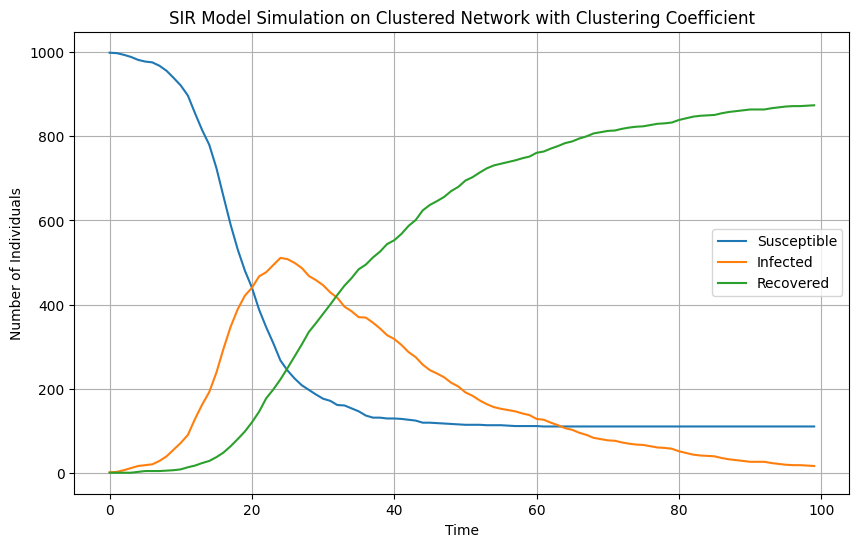
\includegraphics[width=\linewidth]{Figures/analysis_4_cc_0.15.png}
        \caption{SIR Model Simulation on Clustered Network with Clustering Coefficient}
        \label{analysis_4_sne_1}
    \end{minipage}
    \hspace{0.05\textwidth}
    \begin{minipage}[t]{0.45\textwidth}
        \centering
        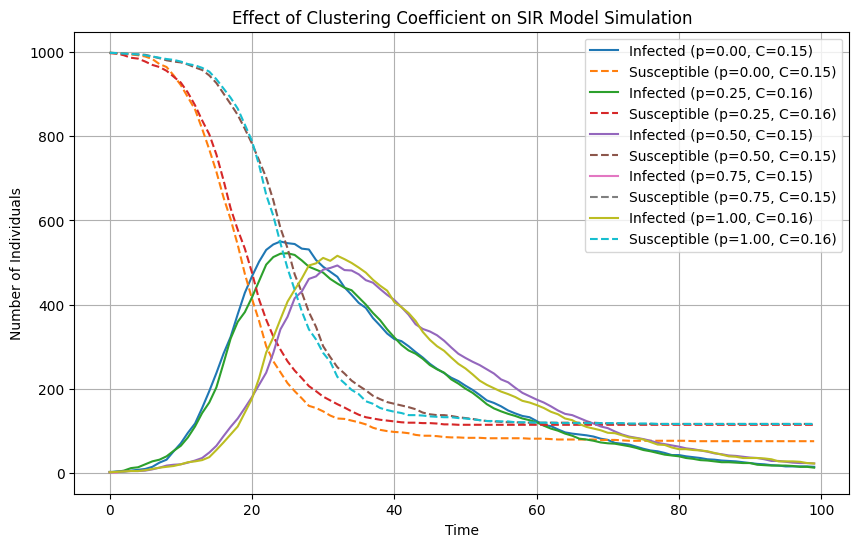
\includegraphics[width=\linewidth]{Figures/analysis_4_c_change.png}
        \caption{Effect of Clustering Coefficient on SIR Model Simulation of Clustered Network}
        \label{analysis_4_sne_change}
    \end{minipage}
\end{figure}

The Clustering Effect on Infection Spread shows that at \( p = 0.00 \), infections quickly die out. As \( p \) increases (e.g., 0.25, 0.50, 0.75, 1.00), infections peak before declining, indicating that higher infection probabilities lead to faster, more widespread transmission (Figure \ref{analysis_4_sne_change}). A larger clustering coefficient (\( C = 0.16 \)) prolongs the infection duration due to more efficient spread within closely connected social groups, while lower clustering results in quicker but shorter epidemics. Social Interactions play a crucial role—higher clustering keeps infections active longer, while higher infection probabilities \( p \) increase the epidemic's peak magnitude.


\section{Public Health Implications}
In regions with high economic connectedness, broad public health interventions, such as widespread vaccination and social distancing, are essential to mitigate rapid disease transmission across all socioeconomic groups. In contrast, areas with low economic connectedness may benefit more from targeted interventions focused on specific communities, such as low-SES populations where diseases may be more contained.

\textbf{Targeted Interventions:} Public health efforts should prioritize vaccination for high-risk groups identified through Social Network Exposure (SNE) analysis, particularly younger populations acting as key transmitters. Tailored health education campaigns should raise awareness about inter-age group risks and promote preventive measures in high-SNE settings.

\textbf{Flexible Response Strategies:} Public health responses must be adaptive to changes in SNE, implementing temporary restrictions or enhanced measures during community events. Real-time monitoring of SNE can allow for more proactive strategies, enabling health officials to respond dynamically to evolving conditions.

\textbf{Community Engagement:} Encouraging cross-class interactions can strengthen community resilience to outbreaks. Public policies should support initiatives that promote inter-socioeconomic interactions alongside providing essential support services like transportation for older adults to healthcare facilities.

\textbf{Resource Allocation:} Healthcare resources should be allocated based on age-specific risk and SNE patterns. High-SNE areas may require increased medical support due to faster transmission rates, while strategic healthcare infrastructure planning should account for potential spikes in infections among populations frequently interacting across age groups.

\section{Conclusion}
The research presented in this paper highlights the critical role of social network exposure (SNE), connectedness, clustering coefficient, and age-structured dynamics in comprehending and controlling the transmission of infectious diseases. By extending traditional models such as SIR and SLIAR to incorporate SNE, this study demonstrates how cross-class and inter-age interactions accelerate disease transmission, leading to different public health outcomes in various socioeconomic contexts. The simulations of clustered network epidemics highlight the impact of social connections and clustering on disease transmission, providing insights into how closely connected groups may sustain transmission longer.

The findings underscore the need for adaptive and targeted public health strategies, with interventions tailored to specific population dynamics and network structures. These insights have significant implications for vaccine distribution, resource allocation, and community engagement initiatives. Monitoring SNE and integrating it into public health planning can lead to more effective, proactive measures in both highly connected and more isolated regions.

Future research should focus on refining these models with real-world data to validate the findings and explore additional factors, such as mobility patterns and health behaviors, that can influence disease dynamics. Ultimately, a deeper understanding of how social structures impact epidemic spread can inform more efficient and equitable public health policies.

\section{Data and Code Availability}
All data, code, and materials used in this study are available in a GitHub repository for transparency and reproducibility: \href{https://github.com/divya830/Modeling_Disease_Spread_and_Health_Behavior_Diffusion_through_Social_Network_Exposure}{https://github.com/divya830/Modeling\_Disease\_Spread\_and\_Health\_Behavior\_Diffusion\_through\_Social\_Network\_Exposure}. This repository provides access to the full set of resources used in this research.


\begin{small}
\bibliographystyle{IEEEtran}
\bibliography{References}
\end{small}


\end{document}
